\documentclass{article}
\usepackage{amsmath}
\usepackage{graphicx}
\usepackage{listings}
\usepackage{xcolor}
\usepackage{caption}
\usepackage{subcaption}
\usepackage{float}
\graphicspath{{images/}}

\lstset{
    language=Python,
    basicstyle=\ttfamily\small,
    keywordstyle=\color{blue},
    commentstyle=\color{gray},
    stringstyle=\color{red},
    breaklines=true,
    frame=single,
    showstringspaces=false,
}

\title{Building an API for detecting Facial Emotion using FastAPI and PyTorch}
\author{Chanaka Perera, Jason Moore}
\begin{document}

\maketitle 

\section*{Research}

\subsection*{Real-Time Facial Emotion Recognition Using Deep Learning Models}

\begin{enumerate}
    \item \textbf{Convolutional Neural Networks (CNNs)}:
    \begin{itemize}
        \item CNNs are emphasized as the most effective model for facial emotion recognition due to their ability to capture spatial features from images.
        \item CNNs employ convolutional layers with learnable filters to detect patterns like edges and textures.
        \item Techniques such as max-pooling reduce spatial dimensions while retaining significant features.
        \item Fully connected layers map extracted features to emotion classes, leveraging softmax for multi-class classification.
        \item Batch normalization and dropout are incorporated to enhance stability and reduce overfitting.
    \end{itemize}
    \item \textbf{Residual Neural Network (ResNet-50)}:
    \begin{itemize}
        \item ResNet-50, known for its depth (50 layers) and use of residual connections, addresses the vanishing gradient problem.
        \item Its deeper architecture allows it to capture complex features, though at the cost of higher computational requirements.
        \item This model showed lower suitability for real-time tasks due to its resource intensiveness.
    \end{itemize}
    \item \textbf{Recurrent Neural Networks (RNNs)}:
    \begin{itemize}
        \item RNNs handle temporal dependencies in data, suitable for video-based emotion detection.
        \item They process sequences with recurrent connections and internal memory to retain context over time.
        \item Models like LSTM and BLSTM are highlighted for their ability to integrate temporal features for improved emotion recognition.
    \end{itemize}
    \item \textbf{Dual-Temporal Scale CNN (DTSCNN)}:
    \begin{itemize}
        \item This newer architecture uses two convolutional layers with different kernel sizes to capture both local and global patterns in temporal data.
        \item Particularly useful for applications like audio and video emotion recognition.
        \item DTSCNN models achieved good accuracy but require more research to mature.
    \end{itemize}
\end{enumerate}

\subsection*{Comparison and Results}

\begin{itemize}
    \item CNNs outperformed other models in both accuracy and speed, achieving up to 96.03\% accuracy on a modified FER dataset.
    \item ResNet-50, while accurate, was computationally expensive and less suited for real-time tasks.
    \item RNNs excelled in handling temporal features but were less effective for static images.
    \item DTSCNN, though promising, requires further refinement for real-time use cases.
\end{itemize}

\subsection*{Scalable Real-Time Emotion Recognition using EfficientNetV2 and Resolution Scaling}

\subsubsection*{Base Model: EfficientNetV2}
EfficientNetV2 was chosen as the base model as it has a lower computational cost and performs well on a variety of different datasets.
In addition, the model has low inference times and therefore is a great option for a real time solution. [1]

\subsubsection*{Key Techniques}
\textbf{a. Resolution Scaling}
\begin{itemize}
    \item Adjust input resolution to improve accuracy.
    \item More flexibility makes it easier to use on different hardware.
\end{itemize}

\textbf{b. Data Augmentation}
\begin{itemize}
    \item Prior to training images were rotated, flipped, etc: to simulate real world conditions.
\end{itemize}

\textbf{c. Training Setup}
\begin{itemize}
    \item Used pre-trained image-net weights to accelerate training.
    \item Optimized with the Adam optimizer and a dynamic learning rate.
    \item Models trained for 120 epochs on the KDEF dataset.
\end{itemize}

\subsubsection*{Key Points}
\begin{itemize}
    \item \textbf{Real-time Execution:} Real time inference time was determined to be 40 ms.
    \item \textbf{Scalability:} Resolution scaling maintained performance across hardware with varying computational capabilities. It was successfully tested on an Intel-I5 processor.
\end{itemize}

\subsection*{Real-Time Emotional Analysis from A Live Webcam Using Deep Learning}

\subsubsection*{Base Models: MTCNN and VGG-16}
MTCNN was used for face detection while VGG-16 was used for facial emotion recognition classification. [2]

\subsubsection*{Key Techniques}
\textbf{a. Face Detection and Alignment}
\begin{itemize}
    \item Utilized MTCNN to accurately detect and align faces in live webcam feeds.
    \item Ensured consistent face positioning to improve classification accuracy.
\end{itemize}

\textbf{b. Feature Extraction and Classification}
\begin{itemize}
    \item Employed VGG-16 for extracting deep features from facial images.
    \item Applied Transfer Learning to fine-tune the pre-trained VGG-16 model on the FER2013 dataset.
\end{itemize}

\textbf{c. Real-Time Implementation}
\begin{itemize}
    \item Integrated OpenCV for capturing and processing live video streams.
    \item Achieved real-time emotion recognition by optimizing the processing pipeline.
\end{itemize}

\subsubsection*{Key Points}
\begin{itemize}
    \item \textbf{High Training Accuracy:} Achieved 97.23\% accuracy on the training set, demonstrating effective learning of facial emotion patterns.
    \item \textbf{Real-Time Performance:} Successfully implemented a system capable of processing live webcam feeds and displaying emotion classifications in real-time.
    \item \textbf{Hybrid Model Efficiency:} Combining MTCNN and VGG-16 provided a balanced trade-off between speed and accuracy, suitable for real-world applications.
    \item \textbf{Applicability:} Potential applications include patient monitoring, security surveillance, and e-learning environments.
\end{itemize}

\section*{Datasets}

\subsubsection*{FER2013 Dataset}
Based on our findings, we chose to work with the FER-2013 dataset due to its terms of service and availability.
The FER2013 dataset consists of grayscale images of faces, sized at 48x48 px. 
Faces are categorized into one of 7 discrete emotional states:

\begin{itemize}
    \item 0 = Angry
    \item 1 = Disgust
    \item 2 = Fear
    \item 3 = Happy
    \item 4 = Sad
    \item 5 = Surprise
    \item 6 = Neutral
\end{itemize}

The dataset is divided into two main subsets:
\begin{itemize}
    \item \textbf{Training Set:} 28,709 examples
    \item \textbf{Public Test Set:} 3,589 examples
\end{itemize}

\subsubsection*{Other Notable FER Datasets}
The FER-2013 dataset is readily available online and the dataset is relatively small making it an ideal option for small lightweight models.

\textbf{1. CK+ (Extended Cohn-Kanade):}
\begin{itemize}
    \item \textbf{Description:} Contains both posed and spontaneous facial expressions with detailed action units
    \item \textbf{Differences from FER2013:} Better option for dynamic emotional analysis in comparison to the static images available in FER 2013.
\end{itemize}

\textbf{2. JAFFE (Japanese Female Facial Expression):}
\begin{itemize}
    \item \textbf{Description:} Comprises 213 images of Japanese female subjects displaying seven emotions.
    \item \textbf{Differences from FER2013:} Dataset lack data variety and is suitable for specific problems.
\end{itemize}

\textbf{3. AffectNet:}
\begin{itemize}
    \item \textbf{Description:} Large dataset with 1 million samples that are labelled both on the discrete and valence emotion scales.
    \item \textbf{Differences from FER2013:} Data is annotated more richly with more detail
\end{itemize}

\textbf{4. RAF-DB (Real-world Affective Faces Database):}
\begin{itemize}
    \item \textbf{Description:} 30,000 images collected from the net that are labelled according to the 7 basic discrete emotions.
    \item \textbf{Differences from FER2013:} Dataset simulates real world conditions such as different lighting and backgrounds making it a harder but more accurate benchmark.
\end{itemize}

\subsubsection*{Considerations on Dataset Size and Image Resolution}

\textbf{Model Size and Dataset Size}

\begin{itemize}
    \item \textbf{Larger Datasets:} 
    \begin{itemize}
        \item Can support larger and more complex models with several layers and parameters.
        \item Larger dataset means a more varied training set and therefore a better generalized model.
        \item Requires more computation and training time.
    \end{itemize}
    \item \textbf{Smaller Datasets:}
    \begin{itemize}
        \item Works with smaller models.
        \item Can regain performance through techniques like transfer learning and data augmentation.
        \item Good for mobile solutions and when computational resources are limited.
    \end{itemize}
\end{itemize}

\textbf{Reasons for Choosing Smaller Datasets}

\begin{itemize}
    \item \textbf{Resource Constraints:} Used a Google Cloud instance with a T4 GPU (16Gb VRAM) for training and a M3 pro to test inference. 
    \item \textbf{Faster Experimentation:} Smaller datasets allow for quicker training and iteration during the development and tuning of models.
    \item \textbf{Availability and Terms of Service}: FER-2013 dataset is readily available for download on Kaggle hub and is relatively small.
\end{itemize}

\textbf{Impact of Image Resolution on Model Performance and Data Size}

\begin{itemize}
    \item \textbf{Higher Pixel Size (Resolution):}
    \begin{itemize}
        \item Provides more detailed information and can therefore capture more abstract patterns.
        \item Increases the amount of data per image, resulting in larger dataset sizes and higher computational and memory requirements.
        \item Increasing resolution means we need more parameters in the input layers to caputre the data in each pixel and therefore more reousrces.
    \end{itemize}
    \item \textbf{Lower Pixel Size (Resolution):}
    \begin{itemize}
        \item Reduces computational and memory requirements, enabling faster training and inference.
        \item May not capture more complex relationships due to lack of data.
        \item Helps in scenarios where bandwidth or storage is limited, making it easier to manage and process data.
    \end{itemize}
\end{itemize}

\section*{Training a PyTorch Model for detecting facial emotions}

\subsection*{Data Preprocessing}

Training a PyTorch model for detecting emotions involves several key steps, starting with data preprocessing. The following outlines the process and explains the corresponding code used in this project.

\subsubsection*{Overview}

The code used to train the models for inference in this project can be found in the repository under \texttt{./notebooks/FER\_efficientNet.ipynb}. The FER-2013 dataset was used for training and was downloaded directly from KaggleHub.

\subsubsection*{Data Preprocessing}

PyTorch provides built-in functionalities that simplify the preprocessing required for data augmentation.

\begin{verbatim}
train_transform = transforms.Compose([
   transforms.Resize((224, 224)),
   transforms.RandomHorizontalFlip(),
   transforms.RandomRotation(10),
   transforms.ToTensor(),
   transforms.Normalize(mean=[0.485, 0.456, 0.406],
                        std=[0.229, 0.224, 0.225])
])
\end{verbatim}

\paragraph{Explanation:}

\begin{itemize}
    \item \textbf{Resize (224, 224):}
    \begin{itemize}
        \item Purpose: Resizes each input image to 224x224 pixels.
        \item Reason: EfficientNet and other pre-trained PyTorch models like ResNet expect input images of this size. Resizing ensures compatibility, enabling the use of transfer learning.
        \item Impact: While resizing grayscale images (48x48) to a larger size can lead to pixelation, it allows leveraging the powerful feature extraction capabilities of pre-trained models.
    \end{itemize}
    
    \item \textbf{RandomHorizontalFlip:}
    \begin{itemize}
        \item Purpose: Randomly flips the image horizontally with a default probability of 0.5.
        \item Reason: Introduces variability in the training data, helping the model generalize better by learning from different orientations of the same image.
    \end{itemize}
    
    \item \textbf{RandomRotation (10 degrees):}
    \begin{itemize}
        \item Purpose: Randomly rotates the image by up to ±10 degrees.
        \item Reason: Enhances data augmentation by making the model robust to slight variations in face orientation.
    \end{itemize}
    
    \item \textbf{ToTensor:}
    \begin{itemize}
        \item Purpose: Converts the PIL Image or NumPy array to a PyTorch tensor.
        \item Reason: Neural networks in PyTorch operate on tensors. This transformation also scales pixel values from [0, 255] to [0, 1].
    \end{itemize}
    
    \item \textbf{Normalize (mean and std):}
    \begin{itemize}
        \item Purpose: Normalizes the tensor using the specified mean and standard deviation for each color channel.
        \item Values:
        \begin{itemize}
            \item \textbf{Mean}: [0.485, 0.456, 0.406]
            \item \textbf{Standard Deviation}: [0.229, 0.224, 0.225]
        \end{itemize}
        \item Reason: These values are standard for pre-trained models on ImageNet. Normalization ensures that the input data has a similar distribution to the data the model was originally trained on, which can improve convergence and performance.
    \end{itemize}
\end{itemize}

Since the FER-2013 dataset consists of grayscale images (1 channel), but EfficientNet expects 3-channel RGB images, the grayscale images are typically converted to 3 channels by duplicating the single channel. This conversion allows the grayscale images to be compatible with the pre-trained EfficientNet architecture without modifying the input layer.

\subsubsection*{Dataset Splitting}

After defining the transformations, the dataset is split into training, validation, and test sets to ensure effective training and evaluation.

\begin{verbatim}
# Define the path to the dataset
fer2013_path = 'fer2013'

# Create datasets
train_dataset_full = datasets.ImageFolder(root=os.path.join(fer2013_path, 'train'), transform=train_transform)
test_dataset = datasets.ImageFolder(root=os.path.join(fer2013_path, 'test'), transform=val_test_transform)

print(f"Number of training samples (full): {len(train_dataset_full)}")
print(f"Number of test samples: {len(test_dataset)}")
\end{verbatim}

\paragraph{Why Three Separate Sets?}

\begin{itemize}
    \item \textbf{Training Set (22,967 samples):} Used to train the model, allowing it to learn the underlying patterns in the data.
    \item \textbf{Validation Set (5,742 samples):} Used to tune hyperparameters and monitor the model's performance during training, helping to prevent overfitting.
    \item \textbf{Test Set (7,178 samples):} Used to evaluate the final model's performance on unseen data, providing an unbiased assessment of its generalization capabilities.
\end{itemize}

\begin{figure}[htbp]
    \centering
    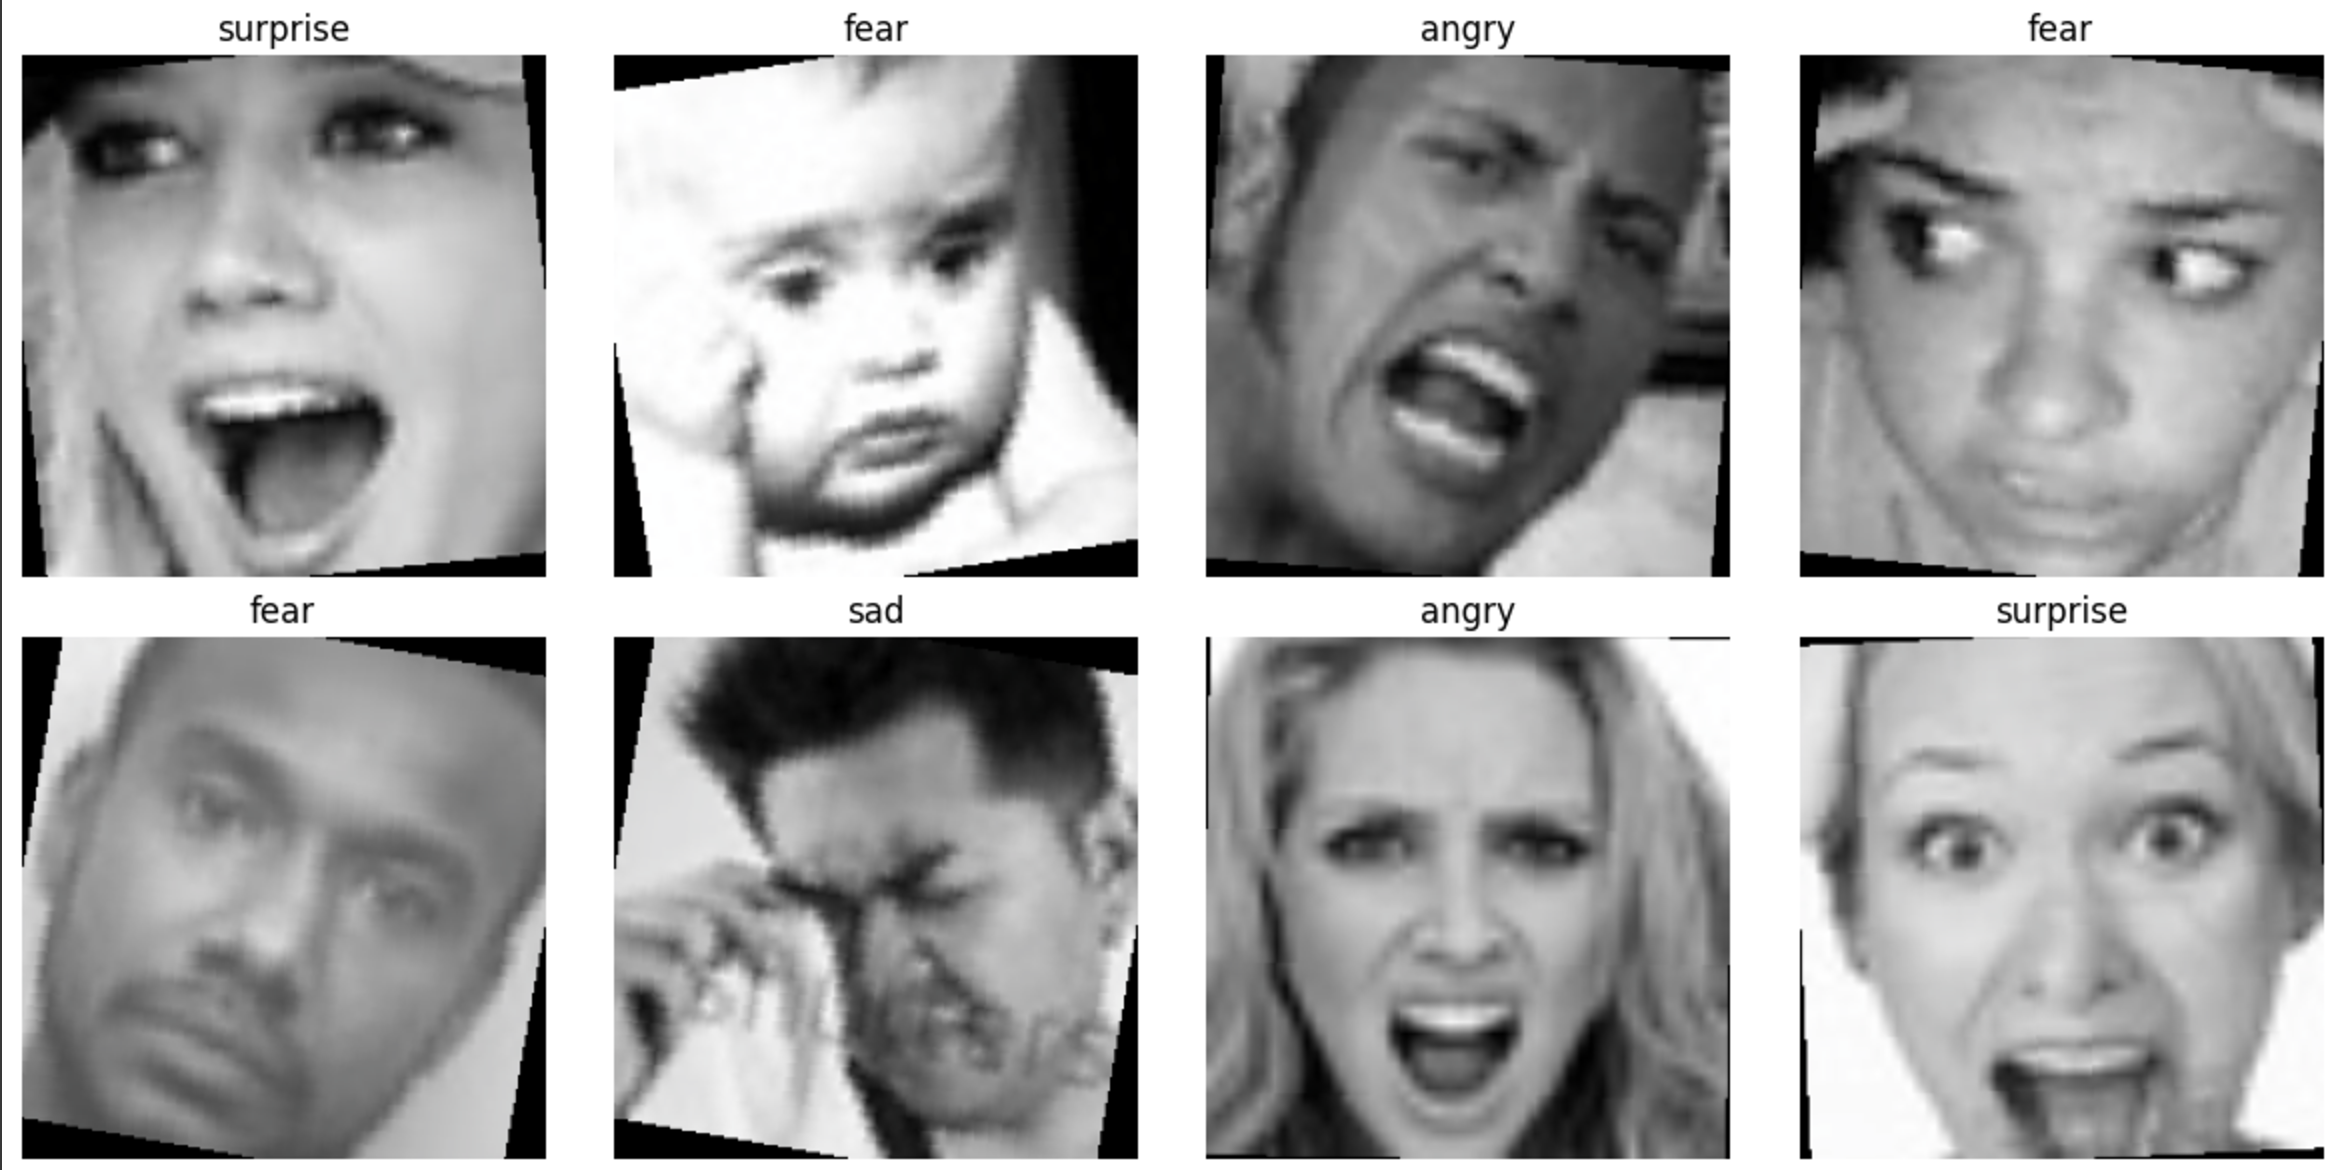
\includegraphics[width=\textwidth]{transformed_images.png}
    \caption{Dataset after pre-processing}
    \label{fig:transformed_images}
\end{figure}

\subsection*{Data Loading}

\begin{verbatim}
# Define DataLoaders with optimized num_workers
batch_size = 64
num_workers = 4
    
train_loader = DataLoader(train_dataset, batch_size=batch_size, shuffle=True, num_workers=num_workers, pin_memory=True)
val_loader = DataLoader(val_dataset, batch_size=batch_size, shuffle=False, num_workers=num_workers, pin_memory=True)
test_loader = DataLoader(test_dataset, batch_size=batch_size, shuffle=False, num_workers=num_workers, pin_memory=True)
    
print("DataLoaders optimized with increased num_workers and pin_memory.")
\end{verbatim}

The provided code sets up DataLoaders in PyTorch, which are essential for efficiently handling and feeding data into the neural network during training, validation, and testing. By defining a \texttt{batch\_size} of 64, the DataLoader groups 64 images together into a single batch. This batching process allows the model to process multiple samples simultaneously, leveraging parallel computation to speed up training and improve computational efficiency. The \texttt{num\_workers} parameter is set to 4, indicating that four subprocesses will be used to load the data in parallel. This parallel data loading minimizes the time the GPU spends waiting for data, ensuring that the training process remains smooth and uninterrupted. Additionally, \texttt{pin\_memory=True} is specified, which enables faster data transfer from the CPU to the GPU by using pinned (page-locked) memory, further optimizing training speed, especially when utilizing CUDA-enabled devices.
\\
During training, the model processes each batch of 64 images, performing forward and backward passes to compute gradients and update the model parameters accordingly. This means that the model's weights are updated after every batch, allowing it to learn from the aggregated information of multiple samples at once. Shuffling is enabled for the training DataLoader (\texttt{shuffle=True}), which ensures that the data is randomized each epoch, enhancing the model's ability to generalize by preventing it from learning the order of the data. In contrast, shuffling is disabled for the validation and test DataLoaders (\texttt{shuffle=False}) to maintain consistency during evaluation, providing a reliable measure of the model's performance on unseen data.

\subsection*{Model Definition}

\begin{verbatim}
class FER2013Model(nn.Module):
    def __init__(self, num_classes=7, pretrained=True):
        super(FER2013Model, self).__init__()
        self.model = EfficientNet.from_pretrained('efficientnet-b0') if pretrained else EfficientNet.from_name('efficientnet-b0')
        # Replace the classifier
        in_features = self.model._fc.in_features
        self.model._fc = nn.Sequential(
            nn.Dropout(p=0.4),
            nn.Linear(in_features, num_classes)
        )

    def forward(self, x):
        x = self.model(x)
        return x

# Check device
device = torch.device("cuda" if torch.cuda.is_available() else "cpu")
print(f"Using device: {device}")

# Initialize the model
model = FER2013Model(num_classes=7, pretrained=True)
model = model.to(device)

print(model)
\end{verbatim}

I defined a custom PyTorch model called the FER2013 model. This class leverages a pre-trained EfficientNet-B0 model from the \texttt{efficientnet\_pytorch} library to take advantage of transfer learning. By setting the \texttt{pretrained} parameter to \texttt{True}, the model loads weights that have been previously trained on the ImageNet dataset, which allows the model to abstract feature representations learned from a large and diverse set of images. This significantly accelerates the training process and improves the model’s performance, especially when dealing with limited datasets like FER-2013. Within the \texttt{FER2013Model} class, the original classifier layer of EfficientNet is replaced with a new sequential module comprising a dropout layer with a probability of 0.4 and a linear layer that maps the input features to the seven emotion classes. This modification tailors the pre-trained model to the specific task of emotion detection by adjusting the final layer to output the correct number of classes.
\\
After defining the model architecture, the code checks for the availability of a CUDA-enabled GPU. CUDA is an API developed by NVIDIA that lets you use the GPU to accelerate training. Since I used a cloud instance that utilized a T4 GPU, I was able to leverage CUDA for this project, significantly speeding up the training.
\\
\subsection*{Model Training}

\begin{verbatim}
# Define loss function
criterion = nn.CrossEntropyLoss()

# Define optimizer - only parameters of the final layer are being optimized initially
optimizer = optim.Adam(model.model._fc.parameters(), lr=1e-3)

def train_epoch(model, loader, criterion, optimizer, device):
    model.train()
    running_loss = 0.0
    correct = 0
    total = 0

    for images, labels in loader:
        images = images.to(device)
        labels = labels.to(device)

        # Zero the parameter gradients
        optimizer.zero_grad()

        # Forward pass
        outputs = model(images)
        loss = criterion(outputs, labels)

        # Backward pass and optimization
        loss.backward()
        optimizer.step()

        # Statistics
        running_loss += loss.item() * images.size(0)
        _, predicted = torch.max(outputs.data, 1)
        total += labels.size(0)
        correct += (predicted == labels).sum().item()

    epoch_loss = running_loss / total
    epoch_acc = correct / total
    return epoch_loss, epoch_acc

def validate_epoch(model, loader, criterion, device):
    model.eval()
    running_loss = 0.0
    correct = 0
    total = 0

    with torch.no_grad():
        for images, labels in loader:
            images = images.to(device)
            labels = labels.to(device)

            # Forward pass
            outputs = model(images)
            loss = criterion(outputs, labels)

            # Statistics
            running_loss += loss.item() * images.size(0)
            _, predicted = torch.max(outputs.data, 1)
            total += labels.size(0)
            correct += (predicted == labels).sum().item()

    epoch_loss = running_loss / total
    epoch_acc = correct / total
    return epoch_loss, epoch_acc

num_epochs = 20
best_val_acc = 0.0

# Lists to store metrics
train_losses = []
train_accuracies = []
val_losses = []
val_accuracies = []

for epoch in range(num_epochs):
    train_loss, train_acc = train_epoch(model, train_loader, criterion, optimizer, device)
    val_loss, val_acc = validate_epoch(model, val_loader, criterion, device)

    train_losses.append(train_loss)
    train_accuracies.append(train_acc)
    val_losses.append(val_loss)
    val_accuracies.append(val_acc)

    print(f"Epoch [{epoch+1}/{num_epochs}] "
          f"Train Loss: {train_loss:.4f} Train Acc: {train_acc:.4f} "
          f"Val Loss: {val_loss:.4f} Val Acc: {val_acc:.4f}")

    # Save the best model
    if val_acc > best_val_acc:
        best_val_acc = val_acc
        torch.save(model.state_dict(), 'best_model.pth')
        print("Best model saved.")
\end{verbatim}

The provided code sets up the loss function and optimizer, and defines the training and validation processes for the emotion detection model. 
The loss function used is \texttt{CrossEntropyLoss}, which is ideal for multi-class classification tasks like emotion recognition as it measures the difference between the predicted class probabilities and the actual class labels.
The optimizer chosen is Adam, an algorithm that adapts the learning rate for each parameter, enhancing convergence speed and overall performance. 
Importantly, the optimizer is configured to update only the parameters of the final classification layer (\texttt{model.model.\_fc.parameters()}) initially. 
This is an application of transfer learning as we leverage the pre-trained layers in EfficientNet-B0 based on the ImageNet dataset.
\\
The \texttt{train\_epoch} function handles the training process for one epoch. It sets the model to training mode and initializes counters for running loss, correct predictions, and total samples. 
For each batch of images and labels from the training DataLoader, the data is moved to the designated device (GPU if available). 
The optimizer's gradients are reset to zero to prevent accumulation from previous iterations. 
The model performs a forward pass to generate predictions, computes the loss using the defined criterion, and then performs a backward pass to calculate gradients. 
The optimizer updates the model's parameters based on these gradients. Throughout the epoch, the function accumulates the loss and counts the number of correct predictions to calculate the average loss and accuracy at the end of the epoch.
\\
Similarly, the \texttt{validate\_epoch} function evaluates the model's performance on the validation set. 
It sets the model to evaluation mode and disables gradient computations to save memory and computational resources. 
The function iterates over the validation DataLoader, performing forward passes to obtain predictions and compute the loss without updating the model's parameters.
It also tracks the total loss and the number of correct predictions to determine the validation loss and accuracy.
\\
I ran this code over 20 epochs which took roughly 2 hours on a T4 cloud instance. The training loss and accuracy over epochs can be seen below:
\begin{figure}[htbp]
    \centering
    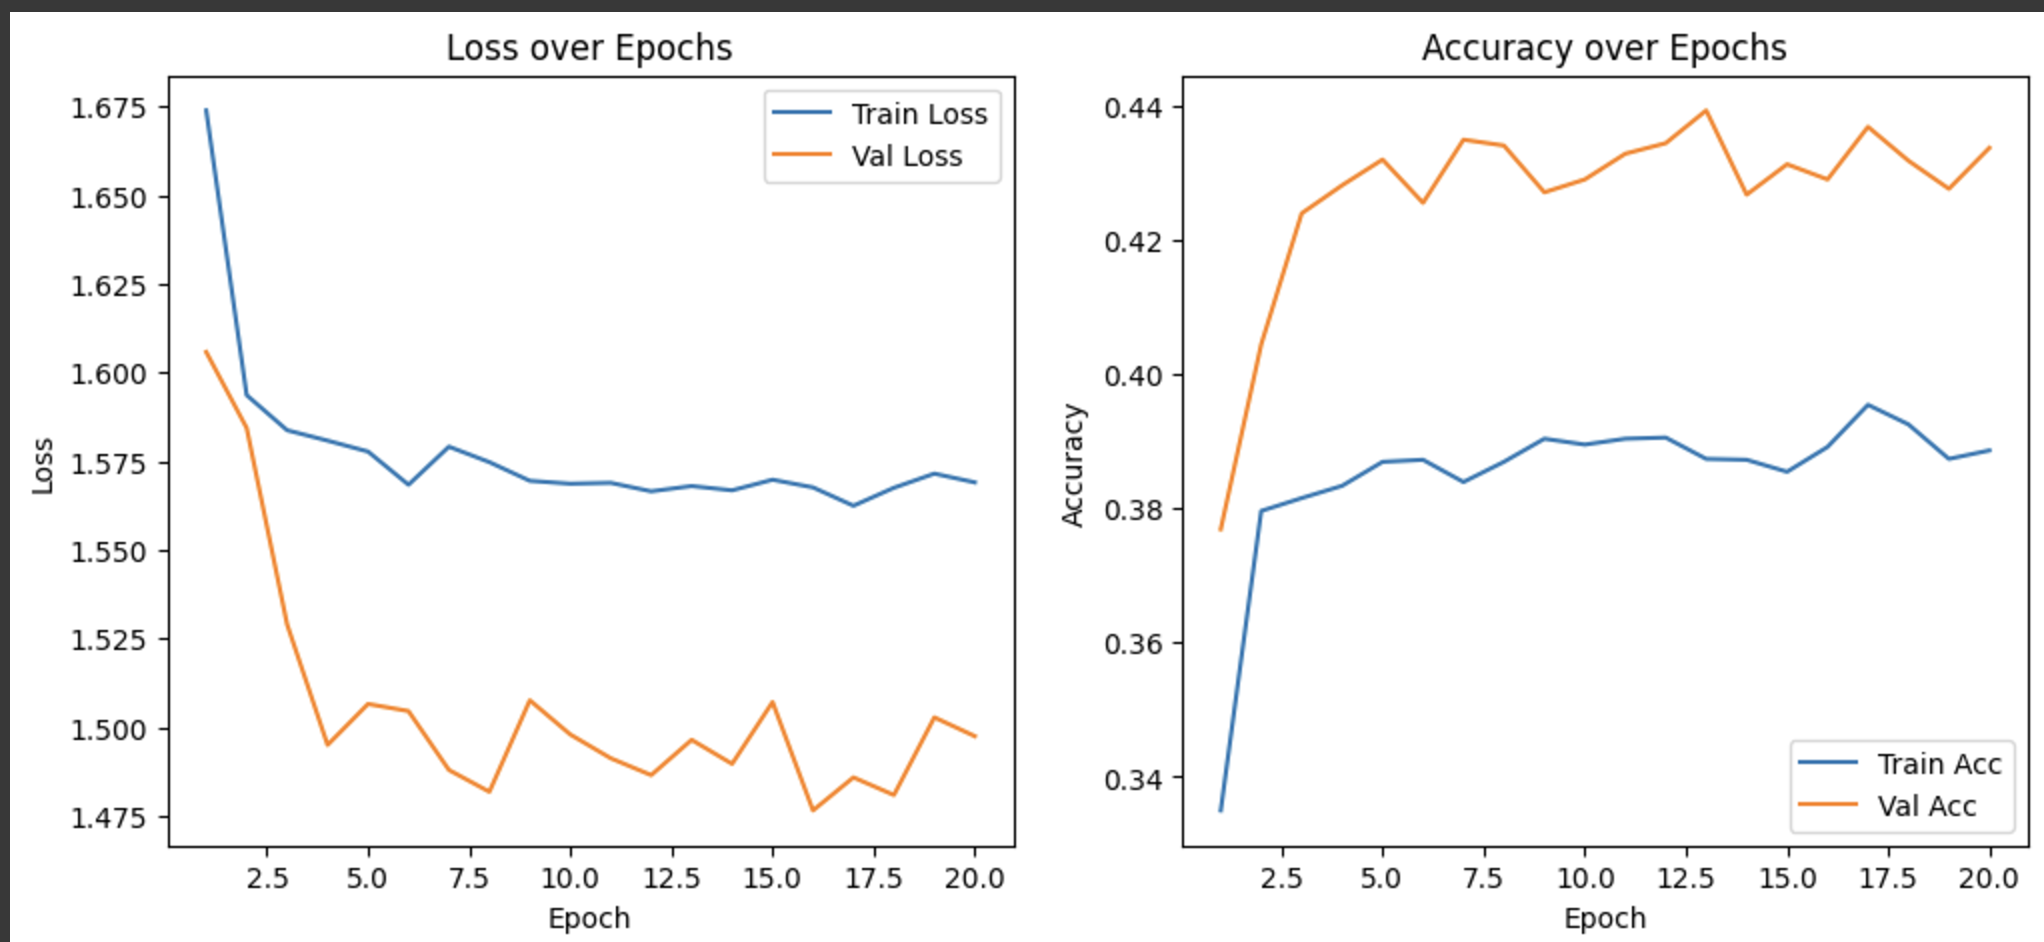
\includegraphics[width=\textwidth]{loss_info.png}
    \caption{Training results}
    \label{fig:training_results}
\end{figure}

\subsection*{Fine-Tuning}

After training we can fine-tune the model to further boost performance. 
Initially, during the training phase, only the parameters of the final classification layer were being optimized while the rest of the model's layers remained frozen.
\\
In the fine-tuning phase, the code first unfreezes all layers of the model by setting \texttt{param.requires\_grad = True} for every parameter in \texttt{model.model.parameters()}.
This action allows the entire network to be trainable, enabling the model to adjust not just the final classification layer but also the deeper layers to better capture the specific features relevant to emotion detection in the FER-2013 dataset.
Alternatively, if resources are limited we can unfreeze a discrete number of layers from the last.
\\
A new optimizer is then defined using Adam with a significantly lower learning rate (\texttt{lr=1e-5}). 
The rationale behind using a lower learning rate during fine-tuning is to make subtle adjustments to the pre-trained weights without causing large updates that could disrupt the valuable feature representations already learned. 
Therefore, a lower learning rate leads to better stability during fine tuning.
The results obtained after fine tuning are plotted below:
\begin{figure}[htbp]
    \centering
    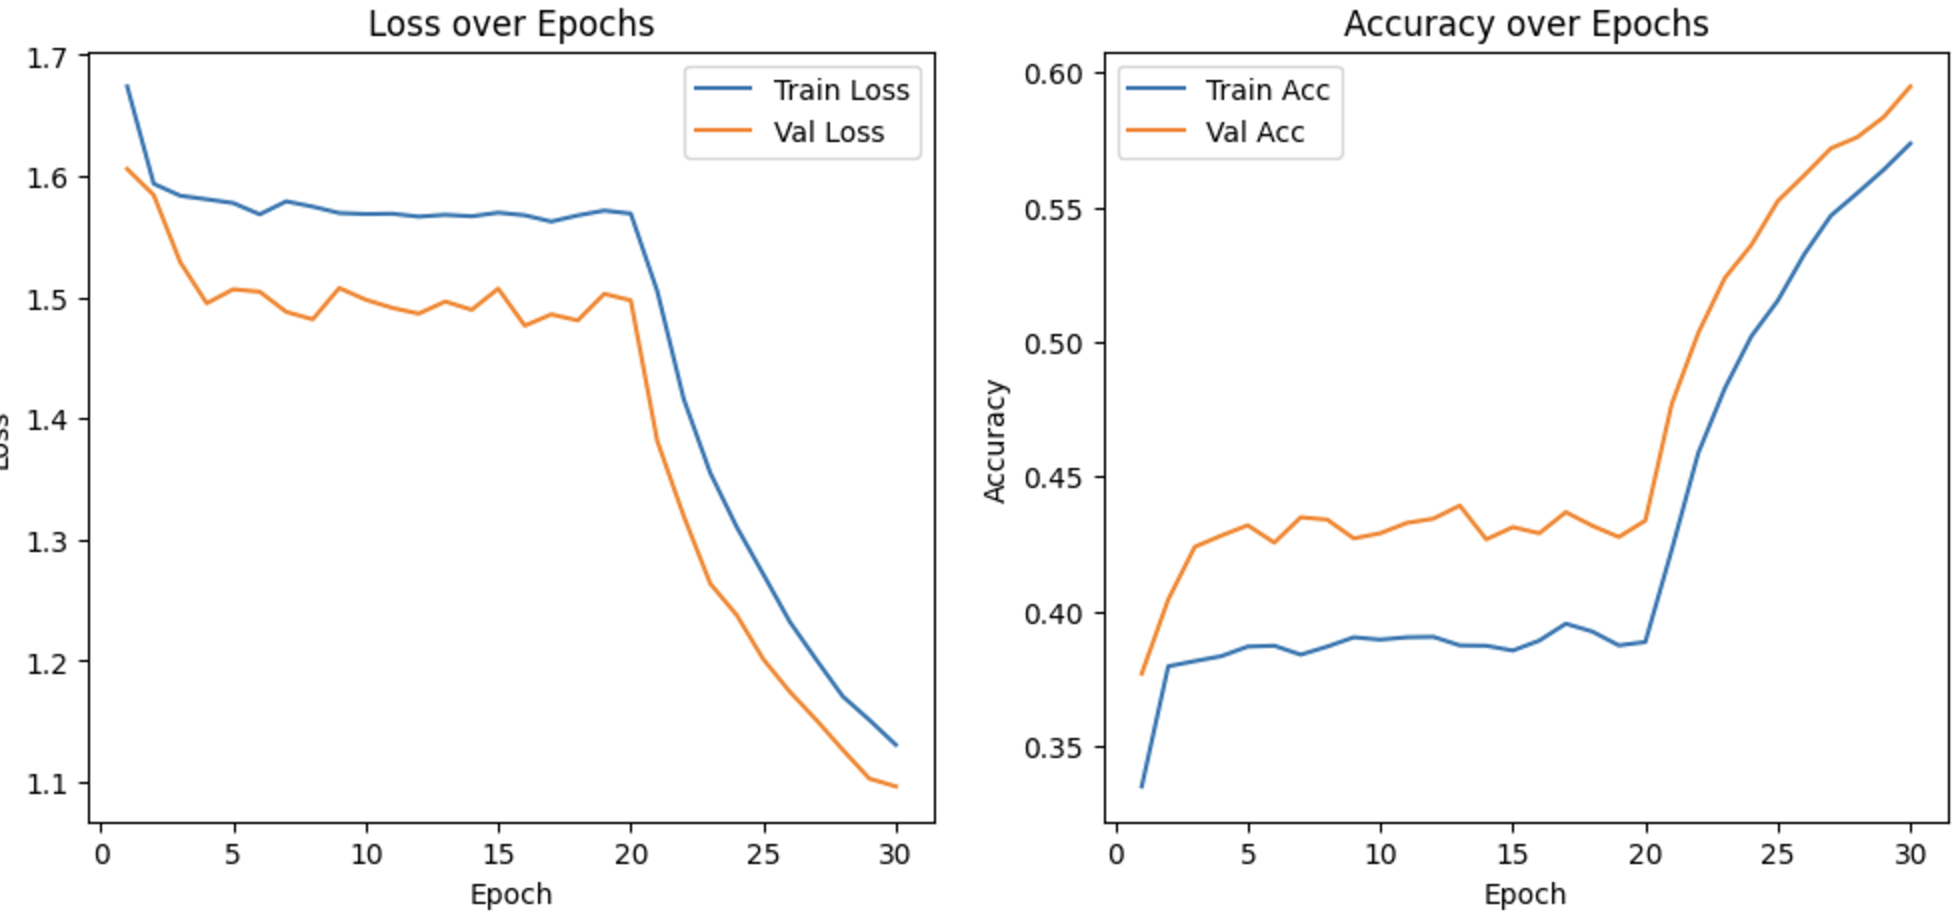
\includegraphics[width=\textwidth]{fine_tuning.png}
    \caption{Training results}
    \label{fig:fine_tuning}
\end{figure}

\subsection*{Results}

The model was evaluated using the test dataset, and a confusion matrix was generated to visualize the performance across different emotion classes. Additionally, a detailed classification report was produced to assess precision, recall, and F1-score for each class.

\begin{verbatim}
Classification Report:
              precision    recall  f1-score   support

      angry       0.45      0.50      0.47       958
    disgust       0.85      0.15      0.26       111
       fear       0.41      0.23      0.30      1024
      happy       0.80      0.83      0.82      1774
    neutral       0.50      0.60      0.54      1233
        sad       0.44      0.48      0.46      1247
   surprise       0.71      0.72      0.72       831

    accuracy                           0.58      7178
   macro avg       0.59      0.50      0.51      7178
weighted avg       0.57      0.58      0.57      7178
\end{verbatim}

\begin{figure}[htbp]
    \centering
    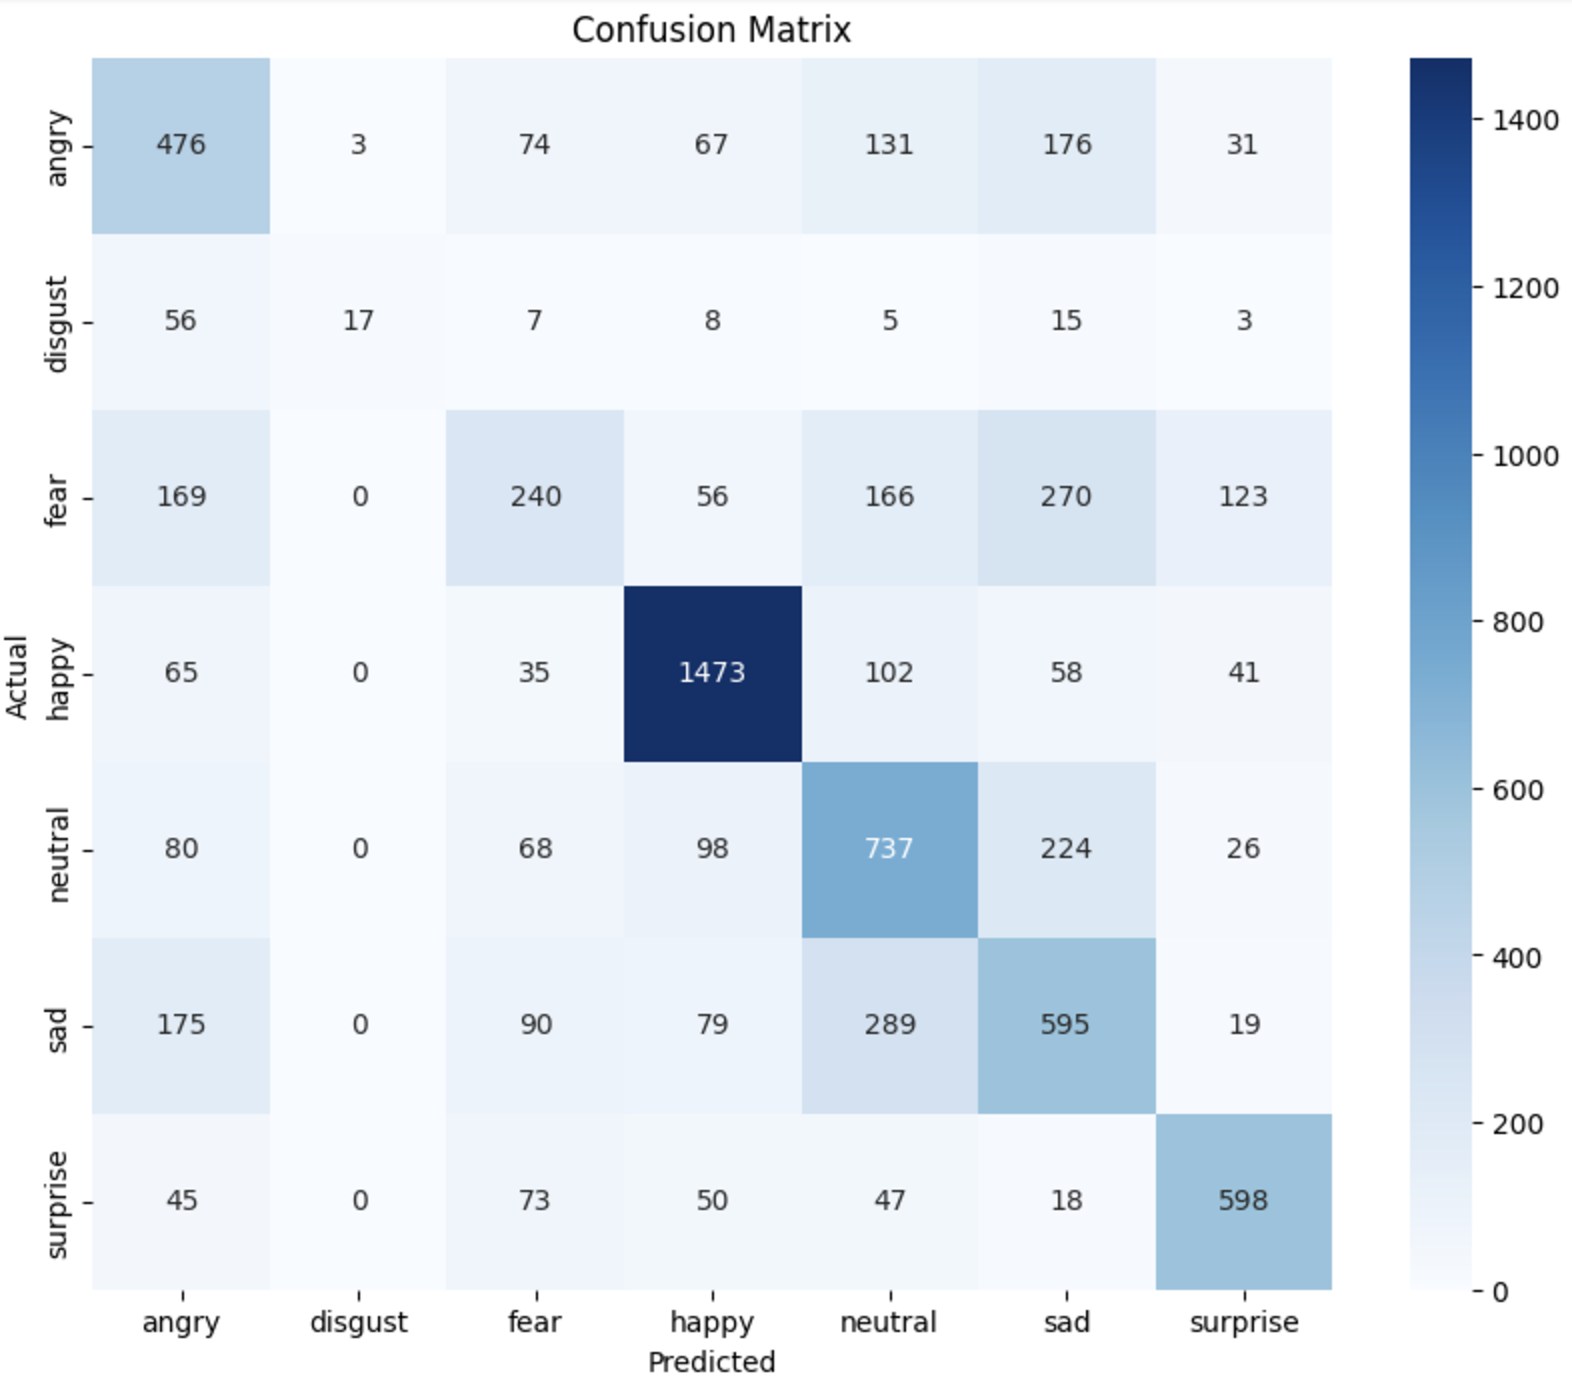
\includegraphics[width=\linewidth]{confusion_matrix.png}
    \caption{Confusion Matrix}
    \label{fig:confusion_matrix}
\end{figure}

The final model had an accuracy of 58\% and performed well in detecting emotions such as happy and neutral and moderately for sad and surprise.
These results indicate that while the model is effective for certain emotions, there is significant room for improvement in others. 
Further training and fine-tuning could enhance the model's ability to accurately detect the less well-performing emotions. However, due to limited computational constraints, this model was chosen as the most viable option for facial emotion recognition.

\section*{REST API}

\subsection*{Preprocessing generic image files}
To create a REST API for detecting emotions using generic images, I utilized FastAPI, a modern web framework for building APIs with Python. The API includes an endpoint named \texttt{predict}, which accepts image files uploaded by users. 
These images can vary widely in size, contain subjects positioned anywhere within the frame, and exhibit different levels of zoom, presenting a challenge since the emotion detection model was specifically trained on centered faces. 
To ensure that the subject's face is properly aligned and standardized for accurate emotion prediction, I integrated Facenet into the preprocessing pipeline.
\\
Facenet, is known for its robust face detection and alignment capabilities, and is based on a Multi-task Cascaded Convolutional Networks (MTCNN) to accurately locate and crop faces within an image, regardless of their position or scale. 
This is essential because the model relies on consistent face positioning to effectively recognize emotions.
Once a face is detected using Facenet, the preprocessing steps involve converting the cropped face image to grayscale to align with the training data specifications, as the emotion detection model was trained on grayscale images. 
To maintain compatibility with the pre-trained EfficientNet architecture, the grayscale image is then converted back to RGB by duplicating the single grayscale channel across all three RGB channels. 
This ensures that the image retains its intensity information while meeting the input requirements of the model.
\\
Subsequently, the image is resized to 224x224 pixels, the standard input size for EfficientNet, ensuring that the model can process the image efficiently during inference.

\begin{figure}[H]
    \centering
    \begin{subfigure}[b]{0.45\textwidth}
        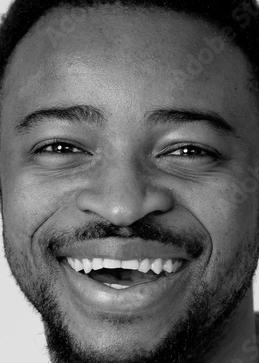
\includegraphics[width=\textwidth]{inference_process}
        \caption{Inference Process}
        \label{fig:inference_process}
    \end{subfigure}
    \hfill
    \begin{subfigure}[b]{0.45\textwidth}
        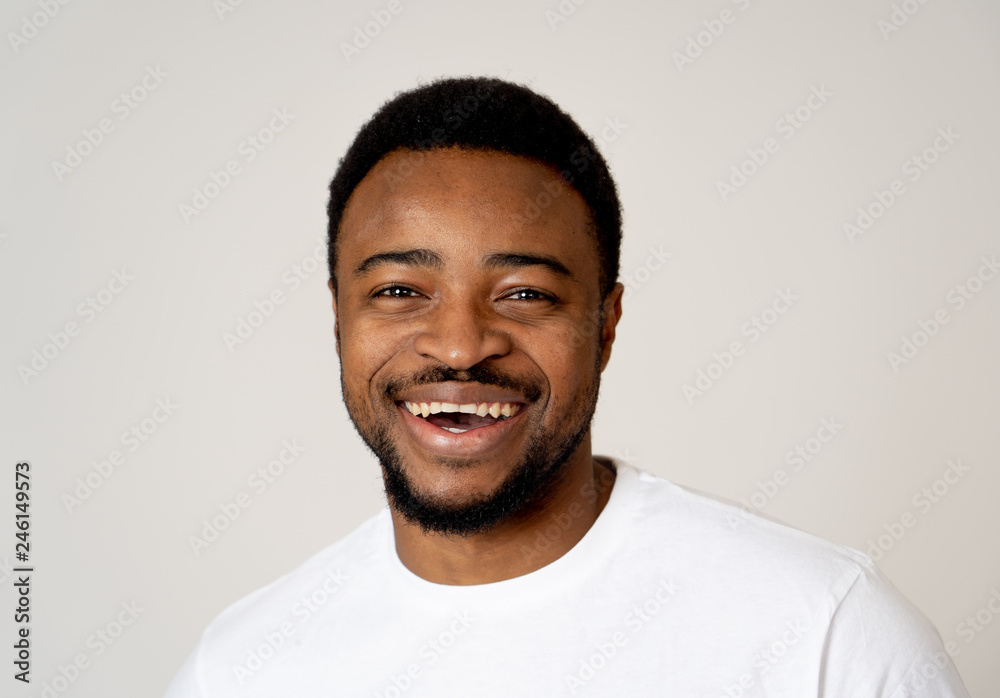
\includegraphics[width=\textwidth]{stock_image}
        \caption{Stock Image}
        \label{fig:stock_image}
    \end{subfigure}
    \caption{Processing images before inference using a MTCNN}
    \label{fig:two_images}
\end{figure}

A MTCNN, unlike a CNN  does more than one thing at a time. It can identify facial features called landmarks. It is also built in stages where each stage is refined based on the previous. Each stage is its own separate neural network forming a cascade.

\subsection*{Testing with POSTMAN}
By combining the two models I was able to generate the API and test with a few stock images.
\begin{figure}[H]
    \centering
    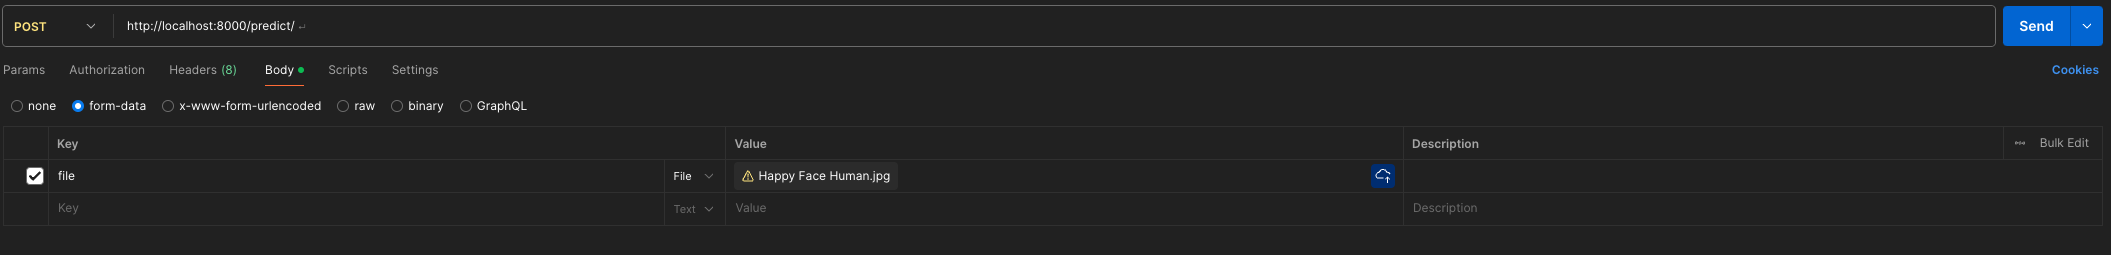
\includegraphics[width=\textwidth]{request.png}
    \caption{API test}
    \label{fig:postman_test}
\end{figure}
\begin{figure}[H]
    \centering
    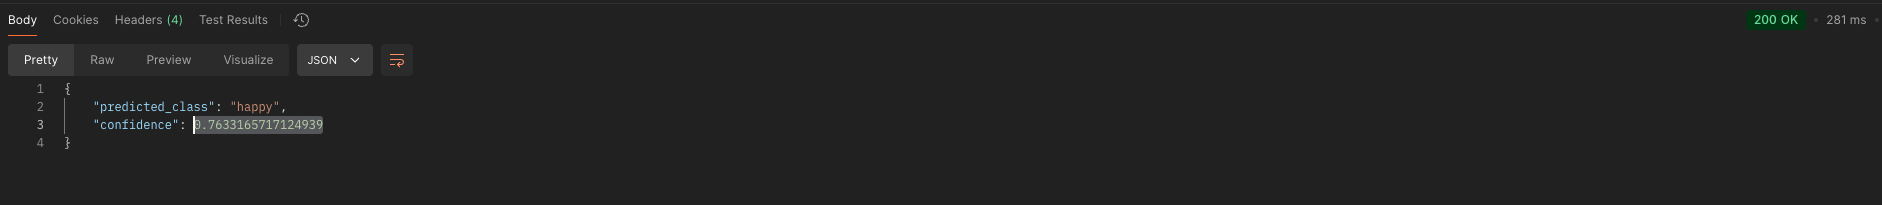
\includegraphics[width=\textwidth]{response.png}
    \caption{API response}
    \label{fig:postman_test2}
\end{figure}

\section*{Key Takeaways}

Throughout this project, we gained a comprehensive understanding of Facial Emotion Recognition (FER) by reading relevant research papers.
We learned how to use PyTorch to train models tailored to specific tasks using a pre-trained model like efficientNet.
We learnt about optimization algorithm like Adam and how it is used during training and fine tuning.
Additionally, We gained insights into pre-processing and augmenting data and how  to fine tune such models for better accuracy.
Utilizing Facenet, We effectively centered faces in images to match the training data requirements.
We also developed a REST API to accept image files, integrating it seamlessly with the emotion detection model. 
Furthermore, We familiarized myself with advanced models such as EfficientNet, ResNet, and Facenet, understanding their architectures and applications in FER.

\section*{References}
\begin{enumerate}
    \item O. Ghadami, A. Rezvanian, and S. Shakuri, "Scalable Real-time Emotion Recognition using EfficientNetV2 and Resolution Scaling," 2024 10th International Conference on Web Research (ICWR), Tehran, Iran, 2024, pp. 1-7, doi: 10.1109/ICWR61162.2024.10533360.
    \item C. A. Kumar and K. Anitha Sheela, "Real-Time Emotional Analysis from A Live Webcam Using Deep Learning," 2022 3rd International Conference for Emerging Technology (INCET), Belgaum, India, 2022, pp. 1-5, doi: 10.1109/INCET54531.2022.9824894.
    \item Naveen, S. Smaran, and A.S. Shamitha, "Real Time Facial Emotion Recognition Using Deep Learning Models," International Journal of Computer Applications (0975 – 8887), vol. 186, no. 29, pp. 41-45, July 2024.
\end{enumerate}

\end{document}
